\chapter{Deadlock Handling}

\section{Introduction}

Deadlock handling is one of the most important topics in Operating Systems and Software Engineering interviews. A deadlock occurs when a set of processes are permanently blocked because each process is waiting for a resource held by another process.

\begin{figure}[H]
\centering
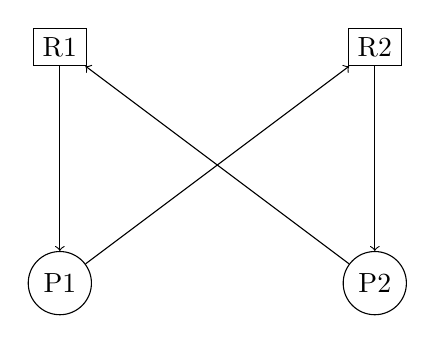
\begin{tikzpicture}
\node[draw,circle] (p1) at (0,0) {P1};
\node[draw,circle] (p2) at (4,0) {P2};

\node[draw,rectangle] (r1) at (0,3) {R1};
\node[draw,rectangle] (r2) at (4,3) {R2};

\draw[->] (p1) -- (r2);
\draw[->] (r2) -- (p2);
\draw[->] (p2) -- (r1);
\draw[->] (r1) -- (p1);
\end{tikzpicture}
\caption{Deadlock Cycle}
\end{figure}

\section{Deadlock Prevention}

Deadlock prevention ensures that at least one of the four necessary conditions for deadlock never holds.

\subsection{Necessary Conditions}

\begin{enumerate}
\item Mutual Exclusion
\item Hold and Wait
\item No Preemption
\item Circular Wait
\end{enumerate}

\subsection{Prevention Techniques}

\begin{longtable}{|p{4cm}|p{9cm}|}
\hline
Condition & Prevention Strategy \\
\hline
Mutual Exclusion & Make resources sharable whenever possible \\
\hline
Hold and Wait & Request all resources at once \\
\hline
No Preemption & Allow resource preemption \\
\hline
Circular Wait & Impose resource ordering \\
\hline
\end{longtable}

\section{Resource Ordering}

Assign a unique number to every resource type.

\[
R_1 < R_2 < R_3 < R_4
\]

Processes must request resources in increasing order.

Example:

\[
R_1 \rightarrow R_3 \rightarrow R_4
\]

Allowed.

\[
R_3 \rightarrow R_1
\]

Not allowed.

\subsection{Advantages}

\begin{itemize}
\item Eliminates circular wait
\item Easy to implement
\item Common in databases
\end{itemize}

\section{Resource Preemption}

Resources may be forcibly taken from processes.

\subsection{Example}

\begin{enumerate}
\item P1 holds Printer
\item P2 requests Printer
\item OS preempts Printer from P1
\item Printer assigned to P2
\end{enumerate}

Useful for:

\begin{itemize}
\item CPU scheduling
\item Memory management
\item Virtual machines
\end{itemize}

\section{Deadlock Avoidance}

Deadlock avoidance dynamically analyzes resource allocation requests.

The system grants requests only if the resulting state remains safe.

\section{Safe State}

A safe state guarantees the existence of a safe sequence.

\subsection{Safe Sequence}

A sequence where every process can complete.

Example:

\[
\langle P_1,P_3,P_4,P_0,P_2 \rangle
\]

\subsection{Visualization}

\begin{figure}[H]
\centering
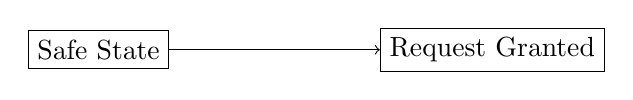
\begin{tikzpicture}

\node[draw] (s1) at (0,0) {Safe State};

\node[draw] (s2) at (5,0) {Request Granted};

\draw[->] (s1)--(s2);

\end{tikzpicture}
\caption{Safe State Transition}
\end{figure}

\section{Unsafe State}

Unsafe state does not necessarily imply deadlock.

However, future requests may lead to deadlock.

\begin{figure}[H]
\centering
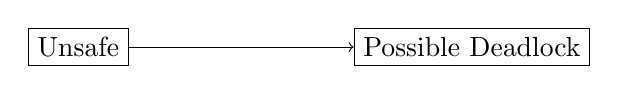
\begin{tikzpicture}

\node[draw] (u1) at (0,0) {Unsafe};

\node[draw] (u2) at (5,0) {Possible Deadlock};

\draw[->] (u1)--(u2);

\end{tikzpicture}
\caption{Unsafe State}
\end{figure}

\section{Banker's Algorithm}

Developed by Edsger Dijkstra.

The algorithm determines whether granting a request keeps the system safe.

\subsection{Data Structures}

\begin{itemize}
\item Available
\item Max
\item Allocation
\item Need
\end{itemize}

Formula:

\[
Need = Max - Allocation
\]

\section{Numerical Example}

\subsection{Available}

\[
(3,3,2)
\]

\subsection{Allocation Matrix}

\begin{center}
\begin{tabular}{cccc}
\toprule
Process & A & B & C\\
\midrule
P0 & 0 & 1 & 0\\
P1 & 2 & 0 & 0\\
P2 & 3 & 0 & 2\\
P3 & 2 & 1 & 1\\
P4 & 0 & 0 & 2\\
\bottomrule
\end{tabular}
\end{center}

\subsection{Max Matrix}

\begin{center}
\begin{tabular}{cccc}
\toprule
Process & A & B & C\\
\midrule
P0 & 7 & 5 & 3\\
P1 & 3 & 2 & 2\\
P2 & 9 & 0 & 2\\
P3 & 2 & 2 & 2\\
P4 & 4 & 3 & 3\\
\bottomrule
\end{tabular}
\end{center}

\subsection{Need Matrix}

\[
Need = Max - Allocation
\]

\begin{center}
\begin{tabular}{cccc}
\toprule
Process & A & B & C\\
\midrule
P0 & 7 & 4 & 3\\
P1 & 1 & 2 & 2\\
P2 & 6 & 0 & 0\\
P3 & 0 & 1 & 1\\
P4 & 4 & 3 & 1\\
\bottomrule
\end{tabular}
\end{center}

\section{Safety Algorithm}

\subsection{Algorithm Steps}

\begin{enumerate}
\item Initialize Work = Available
\item Finish[i] = false
\item Find process whose Need $\leq$ Work
\item Execute process
\item Release resources
\item Update Work
\item Repeat
\end{enumerate}

\subsection{Walkthrough}

Initially:

\[
Work=(3,3,2)
\]

P1 satisfies:

\[
(1,2,2)\leq(3,3,2)
\]

After completion:

\[
Work=(5,3,2)
\]

P3 satisfies:

\[
(0,1,1)\leq(5,3,2)
\]

After completion:

\[
Work=(7,4,3)
\]

P4 satisfies.

After P4:

\[
Work=(7,4,5)
\]

P0 satisfies.

After P0:

\[
Work=(7,5,5)
\]

P2 satisfies.

Safe sequence:

\[
\langle P_1,P_3,P_4,P_0,P_2 \rangle
\]

Therefore state is safe.

\section{Resource Request Algorithm}

Suppose process \(P_i\) requests resources.

\subsection{Checks}

\[
Request_i \leq Need_i
\]

\[
Request_i \leq Available
\]

Temporarily allocate.

Run Safety Algorithm.

Grant only if safe.

\subsection{Example}

Available:

\[
(3,3,2)
\]

Request by P1:

\[
(1,0,2)
\]

Conditions satisfied.

After simulation, system remains safe.

Request granted.

\section{Deadlock Detection}

Instead of preventing deadlocks, the system allows them and periodically detects them.

\subsection{Resource Allocation Graph}

Used when each resource has a single instance.

Cycle implies deadlock.

\begin{figure}[H]
\centering
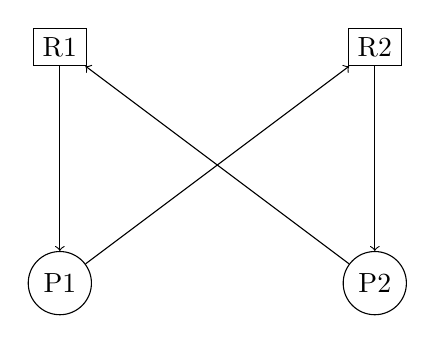
\begin{tikzpicture}

\node[draw,circle] (p1) at (0,0) {P1};
\node[draw,circle] (p2) at (4,0) {P2};

\node[draw,rectangle] (r1) at (0,3) {R1};
\node[draw,rectangle] (r2) at (4,3) {R2};

\draw[->] (p1)--(r2);
\draw[->] (r2)--(p2);
\draw[->] (p2)--(r1);
\draw[->] (r1)--(p1);

\end{tikzpicture}
\caption{Cycle Indicates Deadlock}
\end{figure}

\subsection{Detection Algorithm}

For multiple resource instances:

\begin{itemize}
\item Similar to Banker's Safety Algorithm
\item Detect unfinished processes
\item Report deadlocked set
\end{itemize}

\section{Deadlock Recovery}

After detection, recovery is required.

Two major approaches:

\begin{enumerate}
\item Process Termination
\item Resource Preemption
\end{enumerate}

\section{Recovery by Process Termination}

\subsection{Option 1}

Terminate all deadlocked processes.

Advantages:

\begin{itemize}
\item Simple
\item Immediate
\end{itemize}

Disadvantages:

\begin{itemize}
\item Large loss of work
\end{itemize}

\subsection{Option 2}

Terminate one process at a time.

Factors:

\begin{itemize}
\item Priority
\item Execution time
\item Resources used
\item Remaining execution time
\end{itemize}

\section{Recovery by Resource Preemption}

\subsection{Steps}

\begin{enumerate}
\item Select victim
\item Preempt resources
\item Rollback process
\item Restart later
\end{enumerate}

\subsection{Victim Selection Criteria}

\begin{itemize}
\item Minimum cost
\item Lowest priority
\item Least work completed
\end{itemize}

\section{Flowchart for Deadlock Handling}

\begin{figure}[H]
\centering
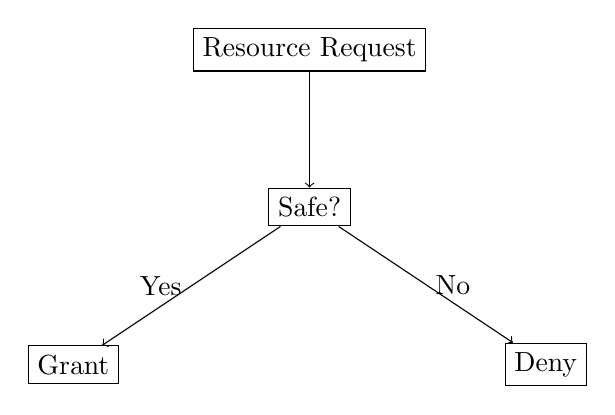
\begin{tikzpicture}

\node[draw] (start) at (0,0) {Resource Request};

\node[draw] (check) at (0,-2) {Safe?};

\node[draw] (grant) at (-3,-4) {Grant};

\node[draw] (deny) at (3,-4) {Deny};

\draw[->] (start)--(check);
\draw[->] (check)--node[left]{Yes}(grant);
\draw[->] (check)--node[right]{No}(deny);

\end{tikzpicture}
\caption{Deadlock Avoidance Decision Flow}
\end{figure}

\section{Practical Deadlock Handling}

Most operating systems use a combination of:

\begin{itemize}
\item Prevention
\item Avoidance
\item Detection
\item Recovery
\end{itemize}

Examples:

\begin{itemize}
\item Linux file locks
\item Windows synchronization objects
\item JVM monitors
\item Database transaction managers
\end{itemize}

\section{Database Deadlock Handling}

Databases frequently encounter deadlocks.

Example:

\begin{itemize}
\item Transaction T1 locks Row A
\item Transaction T2 locks Row B
\item T1 requests B
\item T2 requests A
\end{itemize}

Deadlock occurs.

\subsection{Solutions}

\begin{itemize}
\item Wait-Die
\item Wound-Wait
\item Timeout
\item Deadlock Detection Graph
\end{itemize}

\subsection{Wait-Die}

Older transaction waits.

Younger transaction aborts.

\subsection{Wound-Wait}

Older transaction preempts younger transaction.

\section{Distributed Deadlock Handling}

Deadlocks may span multiple machines.

Challenges:

\begin{itemize}
\item No global clock
\item Distributed resources
\item Communication delays
\end{itemize}

\subsection{Techniques}

\begin{itemize}
\item Centralized Detection
\item Hierarchical Detection
\item Distributed Detection
\end{itemize}

\subsection{Probe-Based Detection}

Special probe messages traverse wait-for graph.

Cycle implies deadlock.

\section{Interview Strategies}

\begin{itemize}
\item Always distinguish prevention, avoidance, detection, and recovery.
\item Know Banker's Algorithm thoroughly.
\item Memorize safe versus unsafe state.
\item Understand database deadlock handling.
\item Explain trade-offs clearly.
\item Practice numerical Banker's Algorithm problems.
\end{itemize}

\section{Common Pitfalls}

\begin{itemize}
\item Unsafe state is not deadlock.
\item Safe state guarantees completion.
\item Deadlock avoidance requires maximum resource information.
\item Prevention may reduce utilization.
\item Recovery can be expensive.
\item Detection incurs runtime overhead.
\end{itemize}

\section{Key Takeaways}

\begin{keytakeaways}
Deadlocks can be handled using prevention, avoidance, detection, and recovery techniques. Resource ordering eliminates circular wait. Banker's Algorithm is the most important avoidance algorithm and relies on safe states and safe sequences. Deadlock detection identifies cycles after they occur, while recovery terminates processes or preempts resources. Databases and distributed systems implement specialized deadlock handling mechanisms due to their unique constraints.
\end{keytakeaways}

\section{Interview Questions with Answers}

\begin{enumerate}
\item What is deadlock handling?\\
Techniques used to prevent, avoid, detect, and recover from deadlocks.

\item What is deadlock prevention?\\
Ensuring at least one deadlock condition never holds.

\item What is deadlock avoidance?\\
Grant requests only if the system remains safe.

\item What is deadlock detection?\\
Finding deadlocks after they occur.

\item What is deadlock recovery?\\
Restoring the system after deadlock detection.

\item What is a safe state?\\
A state with at least one safe sequence.

\item What is an unsafe state?\\
A state that may lead to deadlock.

\item Does unsafe mean deadlock?\\
No.

\item Who developed Banker's Algorithm?\\
Edsger Dijkstra.

\item Purpose of Banker's Algorithm?\\
Deadlock avoidance.

\item Formula for Need?\\
Need = Max - Allocation.

\item What is a safe sequence?\\
Order in which all processes can finish.

\item What is resource ordering?\\
Requesting resources in predefined order.

\item Why use resource ordering?\\
To prevent circular wait.

\item What is resource preemption?\\
Forcibly taking resources.

\item How is deadlock detected with single-instance resources?\\
Resource Allocation Graph cycle.

\item Recovery option 1?\\
Terminate all processes.

\item Recovery option 2?\\
Terminate one process at a time.

\item What is rollback?\\
Returning a process to a previous safe state.

\item Why is prevention expensive?\\
Reduced concurrency.

\item Why is avoidance expensive?\\
Continuous safety checks.

\item Database deadlock technique?\\
Wait-Die.

\item Another database technique?\\
Wound-Wait.

\item Distributed deadlock challenge?\\
No global system state.

\item Most important interview algorithm?\\
Banker's Algorithm.
\end{enumerate}

\section{MCQs with Answers}

\begin{enumerate}
\item Banker's Algorithm is used for:
\begin{enumerate}[label=(\alph*)]
\item Prevention
\item Avoidance
\item Detection
\item Recovery
\end{enumerate}
Answer: (b)

\item Safe state guarantees:
\begin{enumerate}[label=(\alph*)]
\item Deadlock
\item Completion
\item Failure
\item Starvation
\end{enumerate}
Answer: (b)

\item Unsafe state means:
\begin{enumerate}[label=(\alph*)]
\item Deadlock
\item Crash
\item Possible deadlock
\item Restart
\end{enumerate}
Answer: (c)

\item Need matrix equals:
\begin{enumerate}[label=(\alph*)]
\item Allocation-Max
\item Max-Allocation
\item Available-Max
\item Max+Allocation
\end{enumerate}
Answer: (b)

\item Circular wait is prevented by:
\begin{enumerate}[label=(\alph*)]
\item Ordering
\item Paging
\item Scheduling
\item Swapping
\end{enumerate}
Answer: (a)

\item Safe sequence is:
\begin{enumerate}[label=(\alph*)]
\item Execution order
\item Resource type
\item Deadlock graph
\item Scheduler queue
\end{enumerate}
Answer: (a)

\item Resource Allocation Graph cycle indicates:
\begin{enumerate}[label=(\alph*)]
\item Scheduling
\item Deadlock
\item Paging
\item Thrashing
\end{enumerate}
Answer: (b)

\item Detection allows deadlocks to:
\begin{enumerate}[label=(\alph*)]
\item Never occur
\item Occur first
\item Be ignored
\item Be prevented
\end{enumerate}
Answer: (b)

\item Recovery may use:
\begin{enumerate}[label=(\alph*)]
\item Termination
\item Preemption
\item Rollback
\item All of the above
\end{enumerate}
Answer: (d)

\item Resource preemption means:
\begin{enumerate}[label=(\alph*)]
\item Forcefully reclaim resource
\item Allocate memory
\item Swap process
\item Schedule process
\end{enumerate}
Answer: (a)

\item Work vector is used in:
\begin{enumerate}[label=(\alph*)]
\item Safety Algorithm
\item Paging
\item DMA
\item Segmentation
\end{enumerate}
Answer: (a)

\item Finish array stores:
\begin{enumerate}[label=(\alph*)]
\item Completion status
\item Memory size
\item Priority
\item CPU time
\end{enumerate}
Answer: (a)

\item Deadlock prevention removes:
\begin{enumerate}[label=(\alph*)]
\item One necessary condition
\item CPU
\item Process
\item Memory
\end{enumerate}
Answer: (a)

\item Wait-Die is used in:
\begin{enumerate}[label=(\alph*)]
\item Databases
\item Paging
\item Scheduling
\item Networking
\end{enumerate}
Answer: (a)

\item Wound-Wait belongs to:
\begin{enumerate}[label=(\alph*)]
\item Databases
\item Compilers
\item Networking
\item Filesystems
\end{enumerate}
Answer: (a)

\item Probe messages are used in:
\begin{enumerate}[label=(\alph*)]
\item Distributed Detection
\item Paging
\item Caching
\item DMA
\end{enumerate}
Answer: (a)

\item Unsafe state always means deadlock:
\begin{enumerate}[label=(\alph*)]
\item True
\item False
\end{enumerate}
Answer: (b)

\item Dijkstra created:
\begin{enumerate}[label=(\alph*)]
\item Banker's Algorithm
\item LRU
\item FIFO
\item FCFS
\end{enumerate}
Answer: (a)

\item Resource ordering prevents:
\begin{enumerate}[label=(\alph*)]
\item Circular Wait
\item Paging
\item Segmentation
\item Thrashing
\end{enumerate}
Answer: (a)

\item Safe sequence example:
\begin{enumerate}[label=(\alph*)]
\item Ordered completion
\item Memory map
\item Page table
\item Cache entry
\end{enumerate}
Answer: (a)

\item Database deadlock occurs between:
\begin{enumerate}[label=(\alph*)]
\item Transactions
\item Pages
\item Frames
\item Segments
\end{enumerate}
Answer: (a)

\item Recovery by termination:
\begin{enumerate}[label=(\alph*)]
\item Kills process
\item Allocates memory
\item Adds resources
\item Prevents scheduling
\end{enumerate}
Answer: (a)

\item Rollback means:
\begin{enumerate}[label=(\alph*)]
\item Restore earlier state
\item Crash
\item Swap
\item Interrupt
\end{enumerate}
Answer: (a)

\item Safe state implies:
\begin{enumerate}[label=(\alph*)]
\item Completion possible
\item Deadlock certain
\item Starvation
\item Crash
\end{enumerate}
Answer: (a)

\item Distributed deadlocks are difficult because:
\begin{enumerate}[label=(\alph*)]
\item No global state
\item Too much RAM
\item Fast CPU
\item Shared cache
\end{enumerate}
Answer: (a)
\end{enumerate}

\section{Revision Notes}

\begin{revisionnotes}
\item Deadlock handling includes prevention, avoidance, detection, and recovery.
\item Resource ordering prevents circular wait.
\item Safe state guarantees a safe sequence.
\item Unsafe state may lead to deadlock.
\item Banker's Algorithm performs avoidance.
\item Need = Max - Allocation.
\item Safety Algorithm verifies safe states.
\item Detection uses Resource Allocation Graphs and detection algorithms.
\item Recovery uses termination or preemption.
\item Databases use Wait-Die and Wound-Wait.
\item Distributed systems use probe-based detection.
\item Prevention reduces concurrency.
\item Avoidance requires future resource information.
\item Detection introduces runtime overhead.
\item Recovery may lose work.
\end{revisionnotes}

\section{Cheat Sheet}

\begin{longtable}{|p{5cm}|p{8cm}|}
\hline
Concept & Key Idea \\
\hline
Deadlock Prevention & Remove a necessary condition \\
\hline
Deadlock Avoidance & Stay in safe state \\
\hline
Deadlock Detection & Find deadlocks after occurrence \\
\hline
Deadlock Recovery & Restore system operation \\
\hline
Safe State & Safe sequence exists \\
\hline
Unsafe State & May lead to deadlock \\
\hline
Need Matrix & Max - Allocation \\
\hline
Banker's Algorithm & Deadlock avoidance algorithm \\
\hline
Safety Algorithm & Checks system safety \\
\hline
Resource Request Algorithm & Validates requests \\
\hline
Resource Ordering & Prevents circular wait \\
\hline
Preemption & Forcefully reclaim resources \\
\hline
Termination & Kill deadlocked process \\
\hline
Rollback & Restore earlier state \\
\hline
Wait-Die & Older waits, younger aborts \\
\hline
Wound-Wait & Older preempts younger \\
\hline
Distributed Detection & Probe-based cycle detection \\
\hline
Resource Allocation Graph & Deadlock representation \\
\hline
Safe Sequence & Completion order \\
\hline
Interview Focus & Banker's Algorithm \\
\hline
\end{longtable}